\pdfoutput=1
\documentclass[11pt]{article}
\usepackage{ACL2023}
\usepackage{times}
\usepackage{latexsym}
\usepackage[T1]{fontenc}
\usepackage[T5]{fontenc}
\usepackage[utf8]{inputenc}
\usepackage{microtype}
\usepackage{inconsolata}
\usepackage[backend=biber, maxnames=99]{biblatex}
\usepackage{graphicx}
\usepackage{float} 
\usepackage{caption}
\usepackage{xcolor}
\usepackage{subcaption}
\usepackage{soul}
\usepackage{placeins}
\usepackage{makecell} 
\usepackage{hyperref}
\usepackage{lipsum}
\usepackage{minted}
\usepackage{tablefootnote}
\sethlcolor{gray!20}
\addbibresource{refs.bib}
\definecolor{MyGreen}{rgb}{0.0, 0.5, 0.0}
\definecolor{LightGray}{gray}{0.95}
\renewcommand{\thesection}{\arabic{section}.}
\renewcommand{\tablename}{\textbf{Bảng}}
\renewcommand{\thetable}{\textbf{\arabic{table}}}
\renewcommand{\figurename}{\textbf{Hình}}
\renewcommand{\thefigure}{\textbf{\arabic{figure}}}
\renewcommand{\thesubsection}{\thesection\arabic{subsection}.}
\renewcommand{\thesubsubsection}{\thesubsection\arabic{subsubsection}.}
\hypersetup{
    colorlinks=true,
    linkcolor=MyGreen, 
}


\title{Multimodal Sacarsm Detection on Vietnamese Social Media Texts}


\author{Nguyễn Hoàng Hiệp \\
  \texttt{22520452} \\\And
  Nguyễn Duy Hoàng  \\
  \texttt{22520467} \\\And
    Hà Huy Hoàng  \\
  \texttt{22520460}\\}

\begin{document}
\maketitle
\begin{abstract}
Báo cáo này trình bày giải pháp đạt giải Nhì tại bảng B của UIT Data Science Challenge 2024, với bài toán phát hiện sắc thái mỉa mai trong nội dung đa phương tiện. Nhóm đề xuất phương pháp tích hợp dữ liệu văn bản và hình ảnh thông qua các mô hình pretrained được ban tổ chức phê duyệt. Kết quả nghiên cứu thể hiện hiệu quả của phương pháp trong việc nhận diện các yếu tố mỉa mai trong mối tương quan giữa nội dung văn bản và hình ảnh.
\end{abstract}

\section{Giới thiệu}
\hspace*{5mm} Cuộc thi UIT Data Science Challenge 2024 tiếp tục thành công của năm trước, với chủ đề phát hiện sắc thái mỉa mai trong nội dung đa phương tiện (Multimodal Learning), kết hợp giữa văn bản và hình ảnh. Thách thức xoay quanh bốn nhãn phân loại: \textbf{multi-sarcasm}, \textbf{image-sarcasm}, \textbf{text-sarcasm} và \textbf{not-sarcasm}, không chỉ đòi hỏi kỹ thuật cao mà còn thúc đẩy áp dụng trí tuệ nhân tạo vào thực tế, hỗ trợ sàng lọc thông tin chính xác và bảo vệ người dùng trước tin tức không đáng tin cậy.
\\
\hspace*{5mm} Việc sử dụng các mô hình pretrained đang là phương pháp phổ biến trong giải quyết các bài toán machine learning, giúp tiết kiệm thời gian, tài nguyên và nâng cao hiệu quả triển khai. Trong bối cảnh này, các mô hình pretrained cung cấp nền tảng mạnh mẽ cho việc xây dựng hệ thống nhận diện mỉa mai trong nội dung đa phương tiện, đặc biệt khi kết hợp với ngữ cảnh văn bản và hình ảnh.
\\
\hspace*{5mm} Những mô hình này không chỉ mang lại khả năng khởi đầu tốt hơn với những đặc trưng đã được học từ các tập dữ liệu lớn, mà còn tạo điều kiện dễ dàng cho việc tùy chỉnh, tối ưu hóa theo yêu cầu của từng bài toán cụ thể. Với cuộc thi UIT Data Science Challenge 2024, việc ứng dụng và cải tiến các mô hình pretrained hứa hẹn giúp khai phá tiềm năng lớn trong lĩnh vực trí tuệ nhân tạo, từ đó mở rộng khả năng nghiên cứu và ứng dụng công nghệ vào thực tế, đặc biệt trong lĩnh vực xử lý ngôn ngữ tiếng Việt và phân tích nội dung trực tuyến.

\section{Dữ liệu}
\hspace{2mm} Bộ dữ liệu mà ban tổ chức cung cấp cho bài toán này là \textbf{ViMMSD} \footnote{\url{https://www.kaggle.com/datasets/hhhoang/vimmsd-dataset}} và được chia làm 3 phần: \textit{training set}, \textit{dev set}, và \textit{test set}. Các đội tham gia sẽ sử dụng \textit{dev set} để tinh chỉnh (\textit{tuning}) phương pháp của mình và sẽ được đánh giá qua \textit{test set}.  

\hspace{2mm} Mỗi \textit{set} bao gồm một thư mục (được nén dưới dạng \texttt{zip}) chứa các hình ảnh tương ứng và một tệp \texttt{JSON} lưu trữ thông tin cấu trúc như sau:

\begin{verbatim}
    id: { 
        "image": image_path, 
        "caption": caption, 
        "label": label 
    },
\end{verbatim}

\noindent Trong đó:
\begin{itemize}
\vspace*{-2mm}
    \item \texttt{id}: ID của mẫu dữ liệu tương ứng.
    \vspace*{-2mm}
    \item \texttt{image\_path}: Tên tệp hình ảnh được lưu trong thư mục tương ứng với mỗi \textit{set}.
    \vspace*{-2mm}
    
    \item \texttt{caption}: Chú thích (\textit{caption}) của bài đăng tương ứng với hình ảnh (gồm ký tượng chữ cái, chữ số, biểu tượng cảm xúc, ...).
    \vspace*{-2mm}
    
    \item \texttt{label}: Một trong các nhãn thuộc tập (\textit{text-sarcasm}, \textit{image-sarcasm}, \textit{multi-sarcasm}, \textit{not-sarcasm}) trong trainning set hoặc \textit{None} trong dev set và test set.
\end{itemize}
\vspace*{-3mm}
\begin{table}[h!]
\centering
\small\begin{tabular}{|l|c|}
\hline
\textbf{Tập}  & \textbf{Số mẫu} \\ \hline
\texttt{training set} & 10805           \\ 
\texttt{dev set}      & 1413    \\ 
\texttt{test set}     & 1504   \\ \hline
\end{tabular}
\caption{Thông tin bộ dữ liệu}
\label{table:dataset-info}
\end{table}
\vspace*{-5mm}
    
\begin{table}[h!]
\centering

\small\begin{tabular}{|cccc|}
\hline
\textbf{multi-sarcasm}  & \textbf{not-sarcasm} & \textbf{image-sarcasm} & \textbf{text-sarcasm}\\ \hline
4224 & 6062 & 442 & 77\\
\hline
\end{tabular}
\caption{Thông tin số lượng nhãn trong trainning set}
\label{table:dataset-train}
\end{table}



\begin{figure*}[t]
\centering
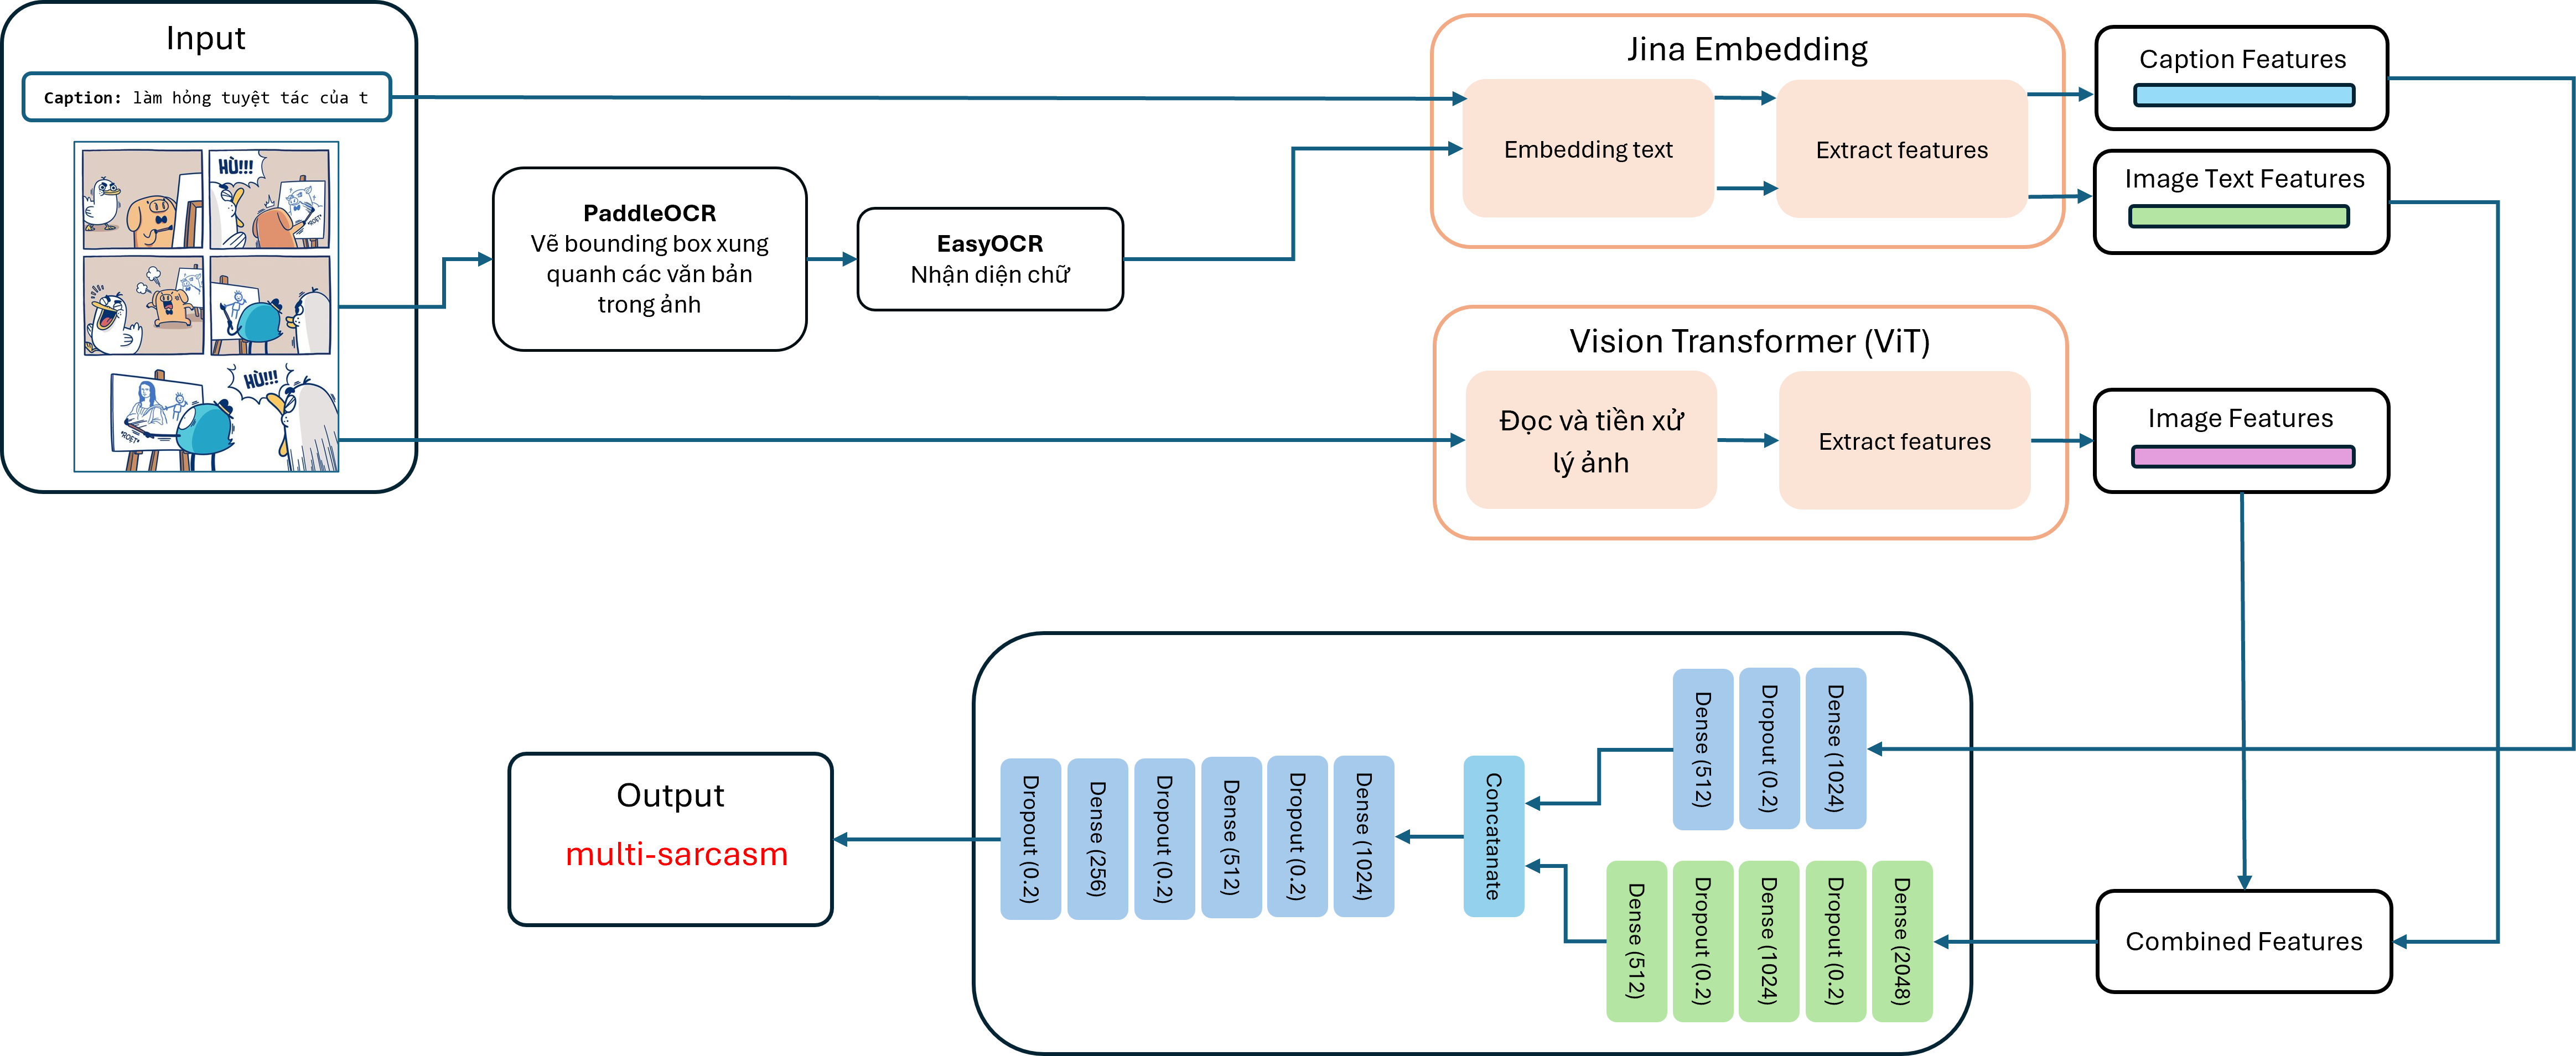
\includegraphics[width=1.0\linewidth]{Picture1.png}
\caption{Kiến trúc mô hình}
\label{fig:example}
\end{figure*}

\FloatBarrier % Giới hạn phần tử nổi tại đây
\section{Kiến trúc}
\hspace*{5mm} Pipeline chính mà nhóm đã dùng cho cuộc thi là kết hợp giữa 4 mô hình pretrained chính: PaddleOCR\cite{paddleocr2020}, EasyOCR\cite{easyocr}, Vision Transformer (ViT)\cite{vit1, vit2} và  Jina Embedding\cite{jinai}. Các feature được trích xuất từ sự kết hợp trên sẽ được đưa qua thêm một mạng neural như trên hình để có thể đưa ra output cuối cùng.
\subsection{PaddleOCR và EasyOCR}
\hspace*{5mm} Trong bài toán này, nhóm đã kết hợp cả PaddleOCR và EasyOCR để tận dụng điểm mạnh của mỗi phương pháp. Thông qua thử nghiệm, nhóm nhận thấy rằng khả năng xác định bounding box của PaddleOCR dường như tốt hơn so với EasyOCR (trong \hyperref[fig:visual]{\textbf{hình}~\ref*{fig:visual}}). Tuy nhiên, khả năng nhận diện văn bản tiếng Việt của PaddleOCR lại chưa đạt chất lượng mong muốn, đặc biệt do các hạn chế trong việc xử lý dấu thanh và mũ của tiếng Việt (như "ă," "â," "ô,"...) trong Hình ().


\begin{figure}[h!]
    \centering
    \begin{subfigure}{0.3\linewidth}
        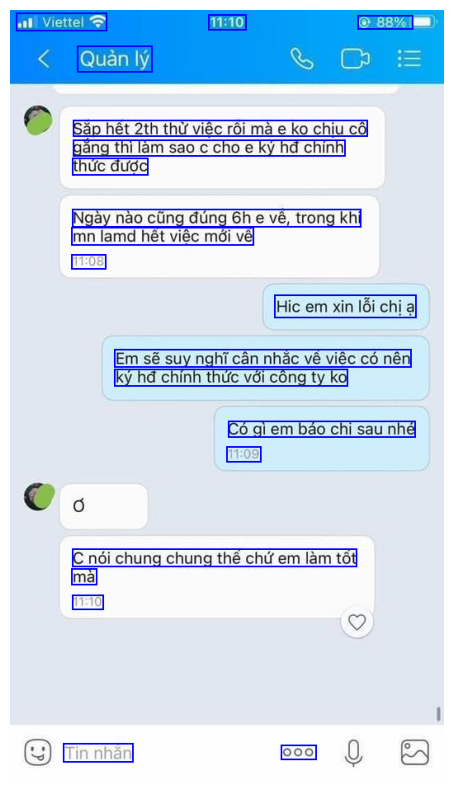
\includegraphics[width=\linewidth]{__results___10_1.png}
        \caption{PaddleOCR}
    \end{subfigure}
    \hfill
    \begin{subfigure}{0.3\linewidth}
        
\includegraphics[width=\linewidth]{__results___10_2.png}
        \caption{EasyOCR}
    \end{subfigure}
    \hfill
    \begin{subfigure}{0.3\linewidth}
        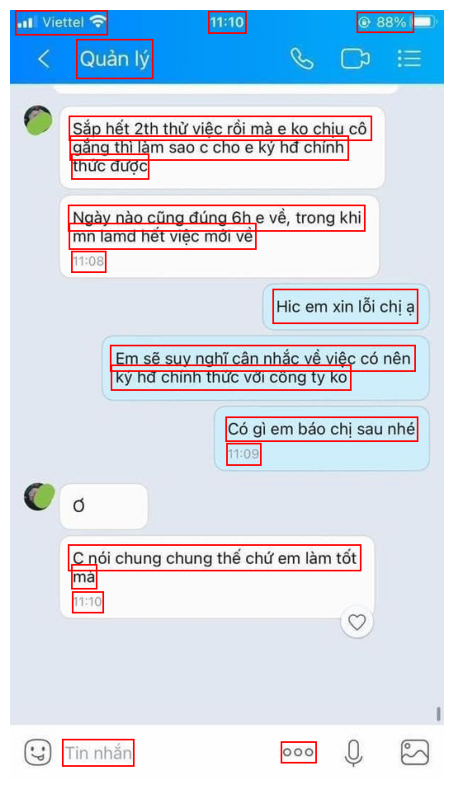
\includegraphics[width=\linewidth]{__results___10_3.png}
        \caption{Combined}
    \end{subfigure}
    \caption{Visualize bounding box}
    \label{fig:visual}
\end{figure}

\vspace*{-3mm}


Do đó, nhóm đã triển khai giải pháp kết hợp như sau: sử dụng bounding box từ PaddleOCR để định vị văn bản, sau đó dùng EasyOCR để nhận diện nội dung. Để cải thiện độ chính xác, nhóm mở rộng các bounding box do PaddleOCR cung cấp. Cụ thể, các bounding box được mở rộng thêm 25\% theo trục y và 1.5\% theo trục x. Việc mở rộng theo trục x chỉ có tác động nhỏ nhưng giúp đảm bảo rằng toàn bộ phần văn bản, bao gồm cả các dấu thanh hoặc mũ, được nhận diện đầy đủ.
\vspace*{-3mm}
\begin{figure}[h!]
    \centering
    \begin{subfigure}{0.3\linewidth}
        
\includegraphics[width=\linewidth]{Picture2.png}
        \caption{PaddleOCR}
    \end{subfigure}
    \hfill
    \begin{subfigure}{0.3\linewidth}
        
\includegraphics[width=\linewidth]{Picture3.png}
        \caption{EasyOCR}
    \end{subfigure}
    \hfill
    \begin{subfigure}{0.3\linewidth}
        
\includegraphics[width=\linewidth]{Picture4.png}
        \caption{Combined}
    \end{subfigure}
    \caption{Kết quả nhận diện dựa trên bounding box}
\end{figure}
\vspace*{-3mm}
\vspace*{-2mm}
\subsection{Vision Transformer (ViT)}
\hspace*{5mm}Vision Transformer (ViT) là một mô hình tiên tiến được thiết kế để học các đặc trưng của hình ảnh bằng cách áp dụng cơ chế tự chú ý (self-attention). Khác với các mô hình CNN truyền thống tập trung vào học các đặc trưng cục bộ từ các vùng nhỏ của ảnh, ViT chia hình ảnh thành các patch (lát) kích thước cố định, mỗi patch được xử lý như một "token" trong chuỗi. Những token này sau đó được nhúng (embedded) vào một không gian đặc trưng, kết hợp với embedding vị trí để bảo toàn thông tin không gian. Với cơ chế tự chú ý, ViT học mối quan hệ giữa các patch một cách toàn cục, giúp mô hình nắm bắt được ngữ cảnh tổng thể và các chi tiết quan trọng trong hình ảnh.

Quá trình tiền xử lý trong ViT bao gồm việc thay đổi kích thước ảnh đầu vào để phù hợp với kích thước cố định của các patch và chuẩn hóa ảnh để đảm bảo tính ổn định trong quá trình huấn luyện. Hình ảnh sau đó được chuyển thành tập hợp các patch không trùng lặp, mỗi patch được flatten thành một vector. Các vector này được ánh xạ tới không gian đặc trưng cao hơn thông qua một lớp dense và kết hợp với embedding vị trí để tạo ra chuỗi đầu vào cho mô hình Transformer.

\begin{figure}[h!]
\centering
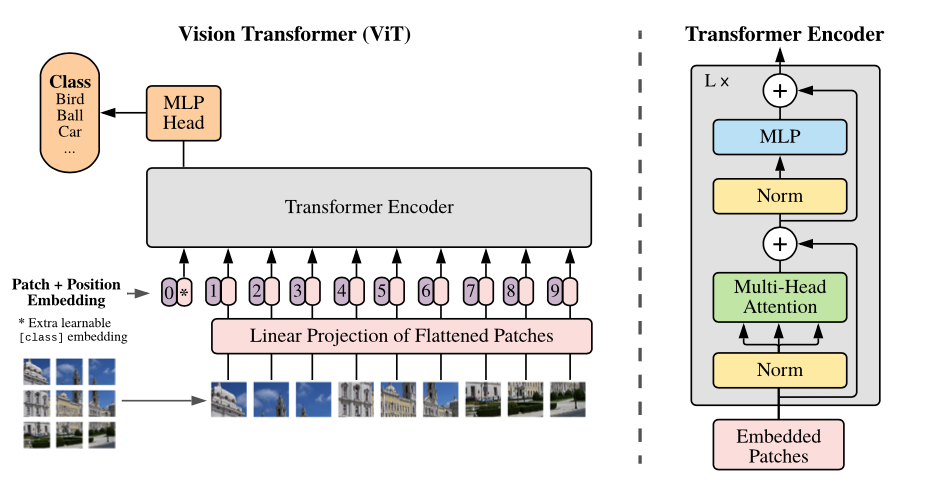
\includegraphics[width=1.0\linewidth]{vit_figure.png}
\caption{Kiến trúc mô hình ViT}
\end{figure}
\vspace*{-5mm}
Trong bài toán này, ViT (\textit{vit-base-patch16-224}) được sử dụng để trích xuất các đặc trưng mạnh mẽ từ hình ảnh, đóng vai trò quan trọng trong việc nắm bắt ngữ cảnh hình ảnh phục vụ cho việc phân tích đa phương thức. Những đặc trưng này được kết hợp với đặc trưng văn bản thông qua một kiến trúc tích hợp, đảm bảo rằng các mối quan hệ phức tạp giữa hình ảnh và ngôn ngữ được khai thác triệt để. Điều này đặc biệt hữu ích khi hình ảnh và văn bản bổ sung ngữ nghĩa cho nhau, một yếu tố quan trọng trong việc hiểu sự mỉa mai.


\subsection{Jina Embedding}

\hspace*{5mm}Trong bối cảnh phát hiện mỉa mai đa phương thức trên dữ liệu mạng xã hội tiếng Việt, việc lựa chọn Jina Embedding như một phương pháp biểu diễn văn bản đóng vai trò then chốt. Jina Embedding nổi bật với khả năng xử lý ngôn ngữ đa dạng, đặc biệt là tiếng Việt, thông qua việc áp dụng kiến trúc transformer được huấn luyện trên tập dữ liệu đa ngôn ngữ quy mô lớn. Điều này cho phép mô hình nắm bắt được các đặc trưng ngữ nghĩa phức tạp và tinh tế trong văn bản tiếng Việt, bao gồm cả những biểu hiện mỉa mai tinh vi thường xuất hiện trên mạng xã hội.

Một ưu điểm đáng kể của Jina Embedding là khả năng tạo ra các vector biểu diễn có độ chính xác cao cho cả văn bản ngắn và dài, phù hợp với đặc điểm đa dạng về độ dài của nội dung mạng xã hội. Mô hình này còn thể hiện hiệu quả vượt trội trong việc xử lý ngữ cảnh và tính đa nghĩa của ngôn ngữ - những yếu tố cốt lõi trong việc nhận diện mỉa mai. Đặc biệt, khả năng tích hợp thông tin ngữ cảnh xuyên suốt câu văn giúp Jina Embedding phân biệt được các sắc thái tinh tế trong cách diễn đạt mỉa mai của người dùng mạng xã hội Việt Nam.

Về quy trình xử lý, Jina Embedding thực hiện một chuỗi các bước tiền xử lý và mã hóa văn bản. Ban đầu, văn bản được chuẩn hóa thông qua việc loại bỏ các ký tự đặc biệt, chuẩn hóa dấu câu và khoảng trắng. Tiếp theo, văn bản được tokenize thành các đơn vị nhỏ hơn, sử dụng bộ tokenizer đa ngôn ngữ được tối ưu hóa cho tiếng Việt. Các token này sau đó được chuyển đổi thành các vector embedding 768 chiều thông qua kiến trúc transformer, trong đó các cơ chế attention đa đầu được sử dụng để nắm bắt mối quan hệ phức tạp giữa các thành phần trong câu, tạo ra biểu diễn vector cuối cùng có khả năng capture được cả ngữ nghĩa tường minh và hàm ý trong văn bản.
\begin{figure}[h!]
\centering
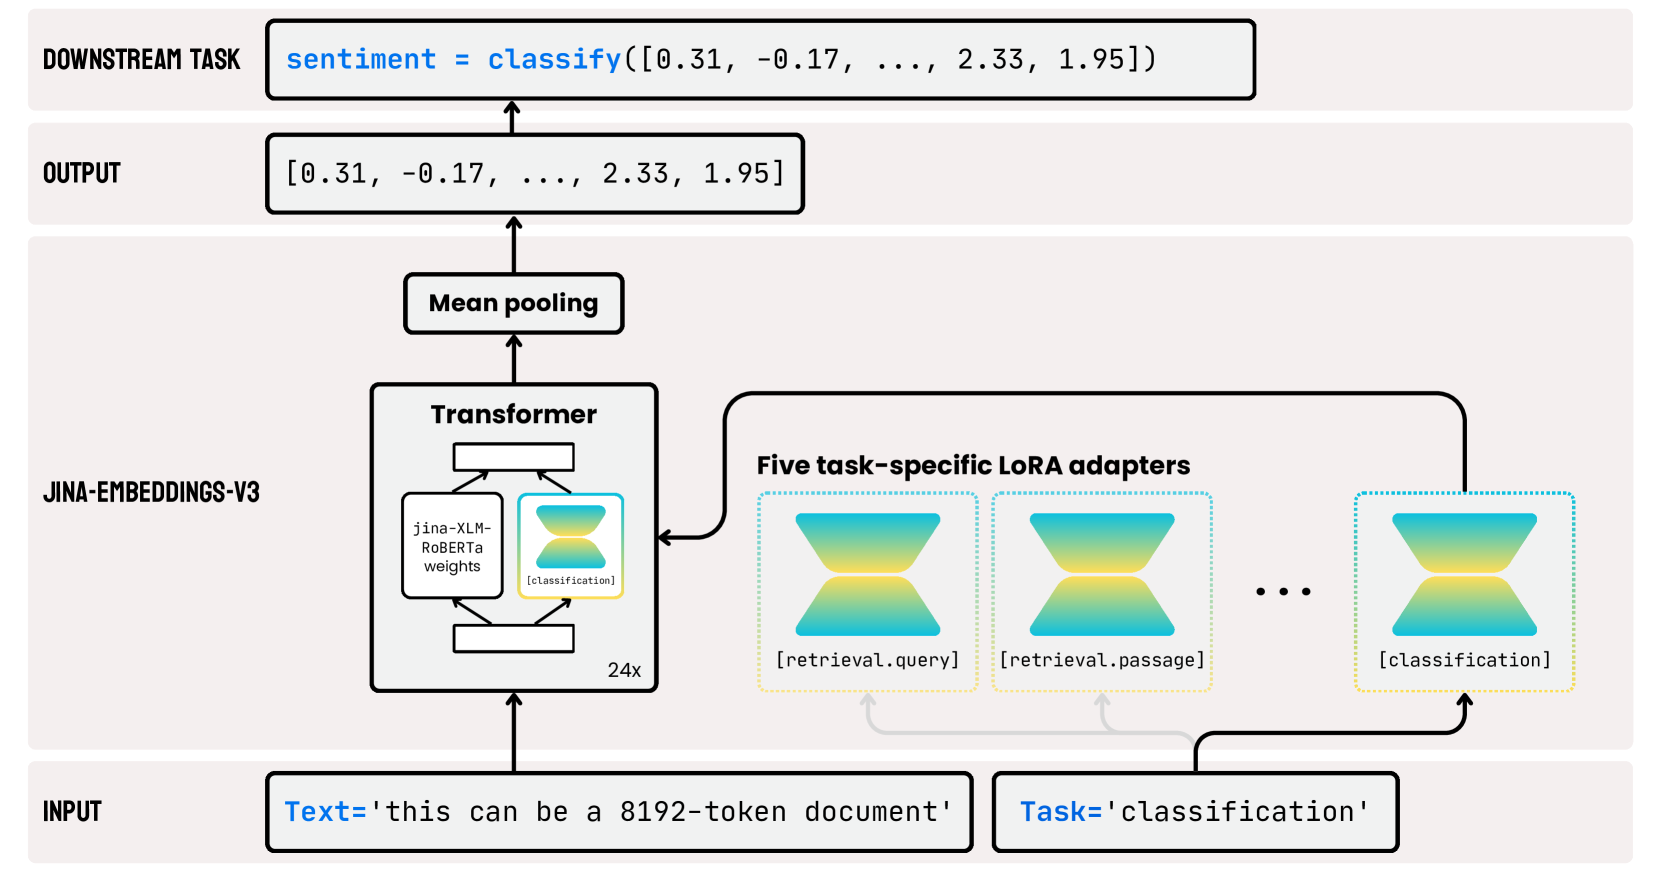
\includegraphics[width=1.0\linewidth]{jina_figure.png}
\caption{Kiến trúc mô hình Jina Embedding}
\end{figure}
\vspace*{-5mm}
\section{Thực nghiệm}
\hspace*{5mm}Trong quá trình tham gia cuộc thi và làm đồ án nhóm đã có thử nghiệm rất nhiều và phát hiện ra được một vài vấn đề 
\subsection{Mất cân bằng dữ liệu}
\hspace*{5mm}Dựa trên \hyperref[table:dataset-train]{\textbf{bảng}~\ref*{table:dataset-train}}, có thể thấy rằng tập dữ liệu huấn luyện có sự mất cân bằng đáng kể giữa các nhãn, với tỷ lệ lần lượt là 39.1\% cho multi-sarcasm, 56.1\% cho not-sarcasm, 4.1\% cho image-sarcasm và 0.7\% cho text-sarcasm. Để giải quyết vấn đề này trong quá trình huấn luyện và dự đoán, nhóm đã áp dụng chiến lược stratified split, đảm bảo tỷ lệ các nhãn trong tập huấn luyện và tập kiểm định được phân bổ đồng đều.

Bên cạnh đó, nhóm sử dụng phương pháp tính trọng số cho các nhãn thông qua compute\_class\_weight, nhằm điều chỉnh trọng số cho từng lớp dữ liệu dựa trên tần suất xuất hiện của chúng. Vì cuộc thi sử dụng F1-macro làm thước đo đánh giá, việc sử dụng compute\_class\_weight giúp tối ưu hóa hiệu suất theo tiêu chí này. Cụ thể, các trọng số được tính toán theo tỉ lệ nghịch với tần suất xuất hiện của mỗi lớp trong tập dữ liệu, theo đó lớp text-sarcasm với chỉ 0.7\% số mẫu sẽ có trọng số cao nhất, trong khi lớp not-sarcasm chiếm 56.1\% số mẫu sẽ có trọng số thấp nhất. Phương pháp này tuy có thể dẫn đến việc hy sinh một phần độ chính xác trên các lớp đa số, nhưng đổi lại giúp mô hình đạt được sự cân bằng tốt hơn trong việc nhận diện tất cả các loại mỉa mai, phù hợp với mục tiêu tối ưu hóa điểm số F1-macro trong cuộc thi.
\vspace*{-2mm}
\subsection{Lựa chọn các đặc trưng}
\hspace*{5mm}Việc sử dụng lớp logits (các giá trị chưa được qua hàm kích hoạt như softmax, đại diện cho các dự đoán thô của mô hình) trong \hl{\textit{"google/vit-base-patch16-224"}} thay cho lớp hidden state cuối cùng có một số lý do hợp lý. Lớp logits giúp giảm thiểu dư thừa thông tin, bởi vì lớp hidden states thường có số chiều lớn và chứa thông tin không cần thiết đối với nhiệm vụ phân loại. Sử dụng logits thay vì hidden states còn giúp giảm chi phí tính toán, đặc biệt là khi số lượng nhãn phân loại nhỏ (chỉ có 4 nhãn trong nghiên cứu này). Kích thước đầu ra của lớp logits có dạng [batch\_size, num\_labels], điều này giúp giảm bớt độ phức tạp của tensor so với các giá trị từ các lớp ẩn trước đó. Trong môi trường huấn luyện với tài nguyên GPU hạn chế, cụ thể là trên nền tảng Kaggle với GPU P100, nhóm gặp phải vấn đề hết bộ nhớ GPU (CUDA out of memory) ngay từ ảnh thứ 650 khi sử dụng lớp hidden states, trong khi không gặp phải tình trạng này khi sử dụng logits. Do đó, để đảm bảo hiệu suất và tiết kiệm bộ nhớ, nhóm đã quyết định sử dụng lớp logits để trích xuất đặc trưng từ mô hình ViT trong suốt quá trình tham gia cuộc thi và làm đồ án.

Bản cuối cùng được nhóm nộp cho ban tổ chức, đạt giải Nhì chung cuộc, sử dụng phương pháp lấy giá trị trung bình (mean pooling) của các đặc trưng từ lớp hidden state cuối cùng của mô hình \hl{\textit{"jinaai/jina-embeddings-v3"}}. Trong khi đó, kết quả thử nghiệm sau cuộc thi chỉ ra rằng việc sử dụng giá trị lớn nhất (max pooling) mang lại điểm số cao nhất (0.4658) trên tập private (test set), vượt xa điểm số của đội đạt giải Nhất (0.4475). Điều này cho thấy phương pháp max pooling có tiềm năng giành giải Nhất nếu được áp dụng.

Tuy nhiên, phương pháp max pooling lại cho kết quả rất thấp trên tập dev set (public test) đều dưới 0.4. Ngược lại, phương pháp mean pooling không chỉ đảm bảo tính ổn định mà còn đạt điểm số 0.4528, giúp nhóm giành vị trí top 1 trong giai đoạn này của cuộc thi còn với test set thì có kết quả thấp hơn (0.4147, ngoài top 5) nhưng vẫn giúp nhóm vẫn có được giải Nhì chung cuộc.

Sự không ổn định của max pooling có thể được giải thích bởi ba yếu tố chính: đặc thù của mỉa mai đòi hỏi sự hiểu biết tổng thể về ngữ cảnh thay vì chỉ tập trung vào các giá trị cực đại của hidden states, hiện tượng overfitting khi max pooling quá tập trung vào một số đặc trưng cụ thể từ tập huấn luyện, và tính đa dạng cũng như phi chuẩn của văn bản mạng xã hội. Trong khi đó, mean pooling, với khả năng tổng hợp toàn diện các hidden states và "làm mịn" các biến thể ngôn ngữ, mang lại kết quả ổn định và nhất quán hơn trên các tập dữ liệu khác nhau.

Ngoài ra nhóm còn thử nghiệm thêm phương pháp lấy token[CLS] nhưng kết quả vẫn thấp hơn việc lấy mean. Phương pháp mean pooling tỏ ra hiệu quả hơn việc sử dụng token [CLS] nhờ khả năng nắm bắt các đặc trưng mỉa mai một cách toàn diện hơn. Token [CLS], được thiết kế để tóm tắt thông tin tổng thể của câu, thường không tối ưu trong việc biểu diễn các mối quan hệ phức tạp giữa các từ hoặc cụm từ đặc trưng cho mỉa mai, nhất là trong văn bản mạng xã hội ngắn gọn và phi chính thống. Mean pooling, bằng cách tổng hợp thông tin từ tất cả các hidden states, thể hiện sự linh hoạt trong việc nắm bắt các tương tác giữa văn bản và các đặc trưng liên quan đến hình ảnh. Ngoài ra, do Jina Embedding v3 không được huấn luyện đặc biệt cho tác vụ phát hiện mỉa mai, phương pháp mean pooling – vốn không phụ thuộc vào token cụ thể – thể hiện khả năng tổng quát và ổn định hơn trên các tập dữ liệu khác nhau. Điều này đặc biệt quan trọng khi xử lý dữ liệu mạng xã hội tiếng Việt với đặc trưng ngôn ngữ không chuẩn và biến động cao.
\vspace*{-3mm}
\subsection{Hiệu quả của OCR}
\hspace*{5mm}Nhóm đã thử việc sử dụng pipeline như \hyperref[fig:example]{\textbf{hình}~\ref*{fig:example}} nhưng không sử dụng OCR (đồng nghĩa với việc phải giảm chiều của mạng neural huấn luyện lại) thì được kết quả như \hyperref[table:res-info]{\textbf{bảng}~\ref*{table:res-info}} (hiệu suất được đánh giá bằng F1-macro như cuộc thi). Kết quả cho thấy phương pháp này giúp tối ưu hóa cả hai khía cạnh: định vị và nhận diện văn bản tiếng Việt, đồng thời cải thiện hiệu suất cho bài toán (trên test set).
\vspace*{-3mm}
\subsection{Các vấn đề khác}
\hspace*{5mm}Để giúp giảm hiện tượng dao động mạnh của loss function (ở đây nhóm sử dụng Categorical Cross-Entropy Loss)và giúp quá trình huấn luyện mượt mà và ổn định hơn nhóm đã dùng learning rate schedule theo dạng step decay (giảm learning rate theo bước sau một số epoch nhất định) nhưng loss thấp nhất nhóm từng đạt được trên tập val là 0.7 (bản nộp cho ban tổ chức) lại thấp hơn loss trên tập val là 1.0 (bản tốt nhất đạt điểm cao nhất trên tập test set) có thể nói giá trị loss hay metric (AUC và F1-macro) sử dụng trong trường hợp train không giúp ích được nhiều lắm trong cuộc thi này.

Một trong những thử nghiệm khác là sử dụng các mô hình pretrained khác cho việc trích xuất đặc trưng của caption và chữ trong ảnh như ViSoBERT\cite{visobert} tuy nhiên một điểm yếu của mô hình này là nó chỉ xử lý được 512 token trong khi đó dữ liệu có các caption dài hơn 700 token. 

Ngoài ra, nhóm cũng đã thử label tay cho bộ test set kết quả khá là bất ngờ khi tự label thì điểm F1-macro trả về chỉ có khoảng 0.45. Việc định nghĩa một ảnh hoặc caption có tính mỉa mai hoặc châm biếm (sarcastic) hay không được định nghĩa như sau bởi ban tổ chức:
\vspace*{-3mm}
\begin{itemize}
    \item Châm biếm là bất kỳ mẫu nào:
    \vspace*{-2mm}
    \begin{itemize}
        \item Sử dụng phép mỉa mai bằng cách nói ngược lại với ý nghĩa thực sự, đặc biệt để chế nhạo hoặc chế giễu.
        \item Chứa sự không tương xứng giữa văn bản và hình ảnh, thể hiện sự châm biếm thông qua mâu thuẫn hoặc phóng đại.
        \item Sử dụng phép cường điệu để phóng đại hoặc giảm nhẹ thực tế theo cách rõ ràng không có ý định được hiểu theo nghĩa đen.
        \item Kết hợp các hashtag, emoji hoặc dấu câu mang tính châm biếm, thường được sử dụng để truyền tải sự châm biếm trên mạng.
    \end{itemize}
    \vspace*{-2mm}
    \item Không châm biếm là bất kỳ mẫu nào:
    \vspace*{-2mm}
    \begin{itemize}
        \item Truyền tải cảm xúc hoặc phát ngôn một cách thẳng thắn và có ý định được hiểu theo nghĩa đen.
        \item Phù hợp trực tiếp với hình ảnh, hỗ trợ cách hiểu theo nghĩa đen của văn bản.
        \item KHÔNG chứa các dấu hiệu ngôn ngữ hoặc hình ảnh thường gắn liền với sự châm biếm.
    \end{itemize}
\end{itemize}  
\vspace*{-3mm}
\hspace*{5mm}Có thể thấy mỉa mai thường mang tính chủ quan, đòi hỏi sự am hiểu ngữ cảnh hoặc sắc thái văn hóa nhất định. Người gán nhãn có thể thiếu sự nhất quán hoặc bị ảnh hưởng bởi cách hiểu cá nhân, dẫn đến việc gán nhãn không đồng nhất trong các tập dữ liệu được cung cấp. Ngoài ra, mô hình có khả năng học được các đặc trưng trừu tượng mà con người khó nhận ra, trong khi quá trình tự gán nhãn dễ bị sai sót do thiếu sự nhất quán, hạn chế về thời gian, và các yếu tố tâm lý như mệt mỏi hoặc thiên kiến cá nhân. Những yếu tố này dẫn đến kết quả tự gán nhãn thiếu chính xác và ổn định so với mô hình đã được tối ưu hóa.

Một điều nữa là nhóm không tiền xử lý bất cứ dữ liệu nào kể cả ảnh lẫn chữ bởi vì các mô hình pretrain đã làm việc đó rồi. Nhưng Jinai Embedding lại không loại stopwords, không lemmatization/stemming, không lowercase toàn bộ text như các mô hình phổ biến khác và đó một phần lí do nhóm chọn mô hình này bởi vì Jinai Embedding được thiết kế để hiểu được ngữ cảnh tự nhiên của ngôn ngữ, nắm bắt được các sắc thái và ý nghĩa tinh tế.

\begin{table}[h!]
\centering
\small\setlength\tabcolsep{4pt} % Giảm khoảng cách giữa các cột
\begin{tabular}{|>{\arraybackslash}m{5cm}|c|c|}
\hline
\textbf{Thử nghiệm} & \textbf{dev set} & \textbf{test set} \\ \hline
\texttt{-OCR +mean $\rightarrow$ caption} & 0.4121 & 0.4042 \\ 
\texttt{+OCR +CLS $\rightarrow$ caption, text} & 0.4091 & 0.4037 \\ 
\texttt{+OCR +weighted $\rightarrow$ caption, text} & 0.4299 & 0.3643 \\ 
\texttt{-OCR +CLS $\rightarrow$ caption} & 0.3901 & 0.3996 \\ 
\texttt{+OCR +CLS $\rightarrow$ caption, mean $\rightarrow$ text} & 0.4117 & 0.405 \\ 
\texttt{+OCR +CLS $\rightarrow$ caption, max $\rightarrow$ text} & 0.4022 & 0.3959 \\ 
\texttt{+OCR +mean $\rightarrow$ caption, max $\rightarrow$ text} & 	0.4135 & 0.4037 \\ 
\texttt{+OCR +mean $\rightarrow$ caption, text (nộp BTC)} & 0.4528 & 0.4192 \\ 
\texttt{+OCR +max $\rightarrow$ caption, text (cao nhất)} & 0.4108 & 0.4658 \\
\hline
\end{tabular}
\caption{F1-macro score của các lần thử nghiệm\footnotemark} % Ký hiệu footnote
\label{table:res-info}
\end{table}

\footnotetext{Tất cả các thử nghiệm trên đều dùng chung một mạng neural như pipeline (tất nhiên là số chiều đầu vào dữ liệu sẽ khác nếu không dùng OCR) và chung một learning schedule.} 
\vspace*{-3mm}
Cấu trúc mạng neural không thay đổi trong suốt quá trình thực nghiệm vì nhóm nhận thấy cấu trúc này ổn định và cho ra hiệu suất các thử nghiệm đều ổn:
\vspace*{-1mm}
\begin{figure}[h]
\centering
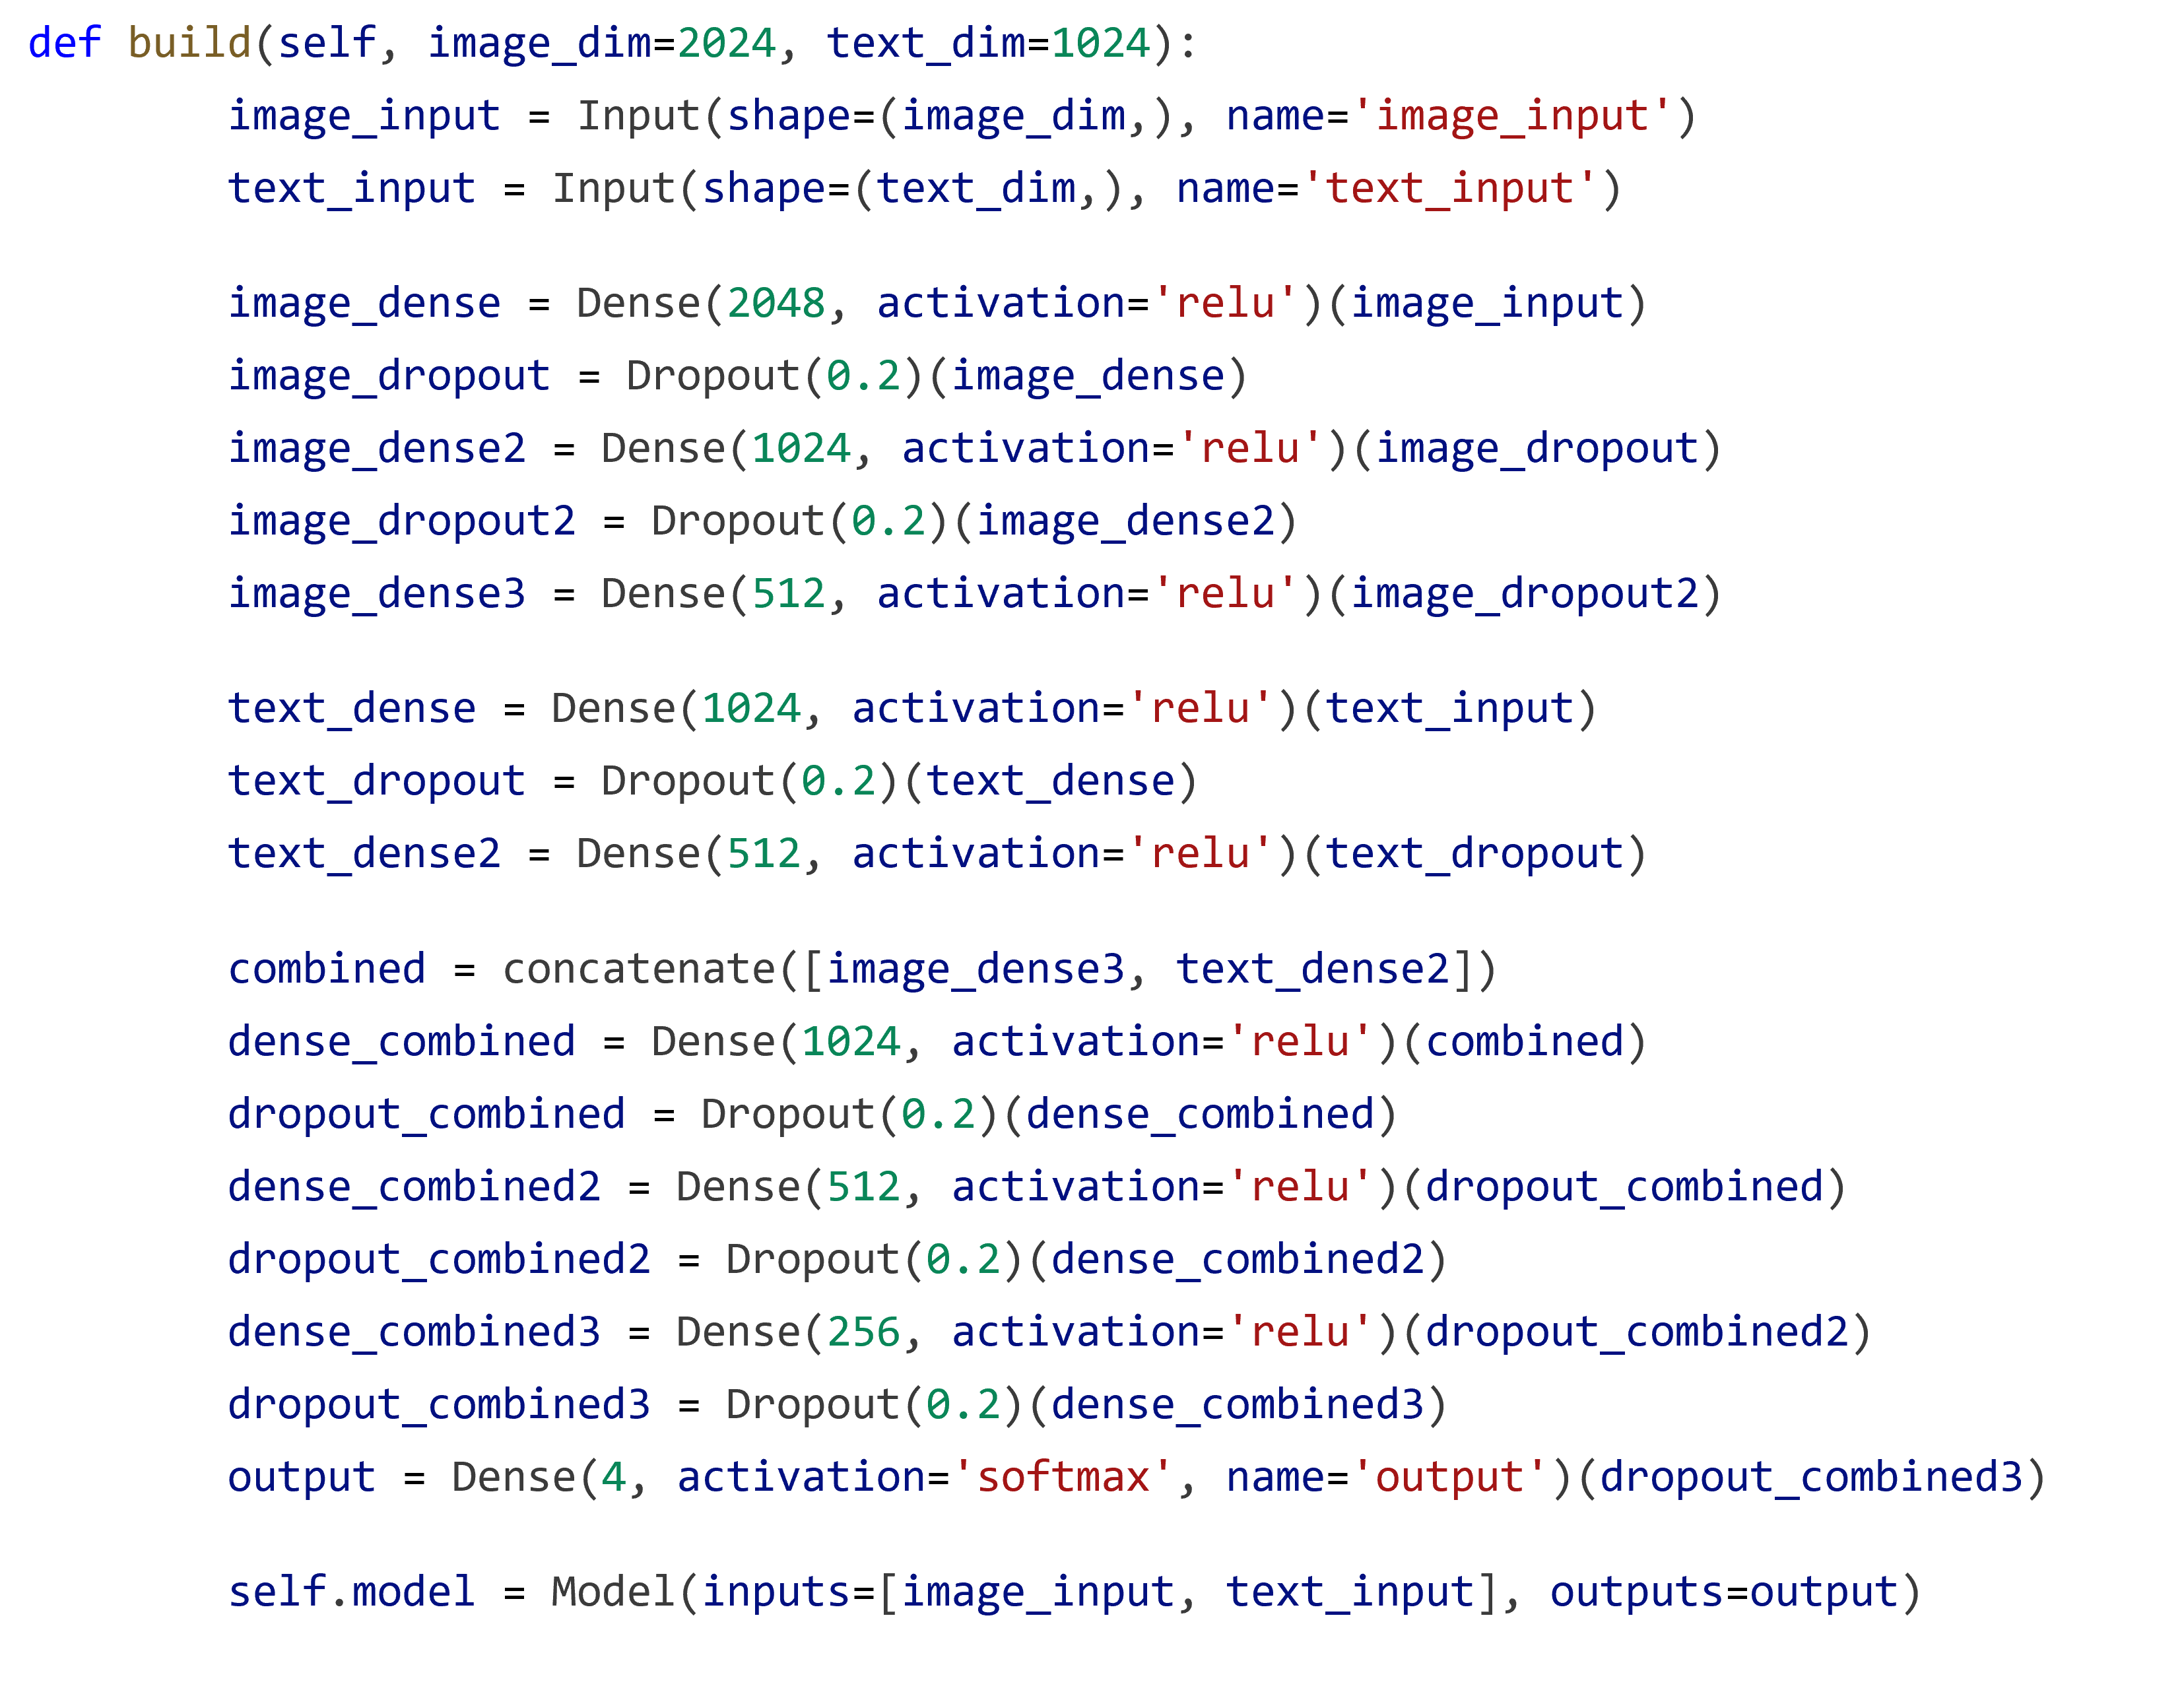
\includegraphics[width=1.0\linewidth]{Picture5.png}
\caption{Kiến trúc mạng neural}
\label{fig:archi}
\end{figure}


\section{Kết luận}
\hspace*{5mm}Qua quá trình tham gia cuộc thi và thực hiện đồ án, nhóm nhận thấy rằng việc lựa chọn các đặc trưng phù hợp và thiết kế kiến trúc mạng neural hợp lý đóng vai trò quan trọng trong việc nâng cao hiệu quả mô hình cũng như khả năng tổng quát hóa trên dữ liệu thực tế.

Để cải thiện bài toán này, nhóm đề xuất một số hướng đi tiềm năng:
\vspace*{-3mm}
\begin{itemize}
\item Xử lý biểu tượng cảm xúc và link URL: Những yếu tố này chứa thông tin ngữ nghĩa quan trọng nhưng bị Jina Embedding bỏ qua. Việc khai thác các đặc trưng này sẽ giúp cải thiện khả năng dự đoán của mô hình.
\vspace*{-3mm}
\item Thử nghiệm các kiến trúc mạng và mô hình tiền huấn luyện mới: Thay đổi các hàm tối ưu, hàm kích hoạt hoặc thử nghiệm các mô hình tiền huấn luyện hiện đại kết hợp kỹ thuật prompting có thể nâng cao hiệu quả xử lý dữ liệu văn bản.
\vspace*{-3mm}
\item Kiểm duyệt và tăng cường dữ liệu: Loại bỏ lỗi nhãn, bất thường trong dữ liệu và áp dụng các phương pháp tăng cường dữ liệu để tăng tính đa dạng và cải thiện độ tổng quát.
\vspace*{-3mm}
\item Chuẩn hóa và sửa lỗi dữ liệu OCR: Xử lý các lỗi chính tả, ký tự không mong muốn từ văn bản trích xuất bằng OCR giúp giảm sai số và tối ưu hóa thông tin đầu vào.
\end{itemize}
\vspace*{-3mm}
Nhóm tin rằng những cải tiến trên sẽ giúp nâng cao hiệu quả bài toán và ứng dụng tốt hơn trong thực tế.

\nocite{*}

\printbibliography[title={Tham khảo}]
\end{document}
